\subsection{题目描述}
Find all integer solutions to the \textbf{Diophantine equation} \( a^5 + b^5 + c^5 + d^5 = e^5 \) within the range \([0, 200]\).
\subsection{程序描述}

1967年,Lander和Parkin使用CDC 6600计算机首次找到方程

\[
    a^5 + b^5 + c^5 + d^5 = e^5
\]

的一个解,即

\[
    27^5 + 84^5 + 110^5 + 133^5 = 144^5
\]

这个解也推翻了欧拉的幂和猜想(即至少需要 \(k\) 个 \(k\) 次幂才能表示另一 \(k\) 次幂的和,且 \(k \geq 2\))。相关参考资料可参见 \href{https://mathworld.wolfram.com/DiophantineEquation5thPowers.html}{Diophantine Equation—5th Powers}。
2004年,J. Frye使用分布式并行计算找到了第二个解:

\[
    55^5 + 3183^5 + 28969^5 + 85282^5 = 85359^5
\]

题目要求我们找到所有满足$0 \leq a \leq b \leq c \leq d < e \leq 200 $的整数解

为了解决这个问题,我们首先采用暴力搜索的方法,遍历所有可能的 \(a, b, c, d, e\) 组合,并逐一检查是否满足方程。在 \texttt{brute\_force.f90} 中实现了这一方法,其伪代码见算法 \ref{alg:bf}。该程序的运行时间达到了8.953秒,速度较为缓慢。

在网络上寻找更优解法时,我偶然发现了一个专门讨论整数幂方程的论坛:\href{http://euler.free.fr/}{Euler Free}。该论坛提到可以通过数论优化的方法。注意到方程中的 \(x^5\) 是齐次的,首先注意到到费马小定理:

\[
    a^{p-1} \equiv 1 \pmod{p}, \quad \gcd(a,p)=1.
\]

基于此,在搜索时可以将步长扩大到5。然而,进一步查阅Lander和Parkin的论文后,未能找到有效的进一步启发。
在Rosetta Code网站上,我发现了C语言中使用的\href{https://rosettacode.org/wiki/Euler%27s_sum_of_powers_conjecture#C}{Mod30 Trick},这让我意识到可以进一步扩展费马小定理的应用范围。
即我们可以证明:

\[
    a^5 \equiv a \pmod{30}
\]

这意味着在搜索时可以将步长扩展到30。(昨天使用这个问题测试过了ChatGPT o1 pre,它枚举证明了所有情况。)
具体而言,对于 \(n = 2, 3, 5\),我们可以分别讨论奇偶性和模数的同余关系:
- 对于 \(n = 2\),由于奇偶性,显然有 \(a^5 \equiv a \pmod{2}\)。

- 对于 \(n = 3\):
- 若 \(\gcd(a, 3) = 1\),则 \(a^2 \equiv 1 \pmod{3}\),因此

\[
    a^5 = a \cdot (a^2)^2 \equiv a \cdot 1^2 \equiv a \pmod{3}
\]

- 若 \(3 \mid a\),则 \(a \equiv 0 \pmod{3}\),因此 \(a^5 \equiv 0 \pmod{3}\)。
- 对于 \(n = 5\):
- 若 \(\gcd(a, 5) = 1\),则 \(a^4 \equiv 1 \pmod{5}\),因此

\[
    a^5 = a \cdot a^4 \equiv a \cdot 1 \equiv a \pmod{5}
\]

- 若 \(5 \mid a\),则 \(a \equiv 0 \pmod{5}\),因此 \(a^5 \equiv 0 \pmod{5}\)。

根据剩余定理,我们立马可以得出:
$a^5 \equiv a \pmod{30}$

利用这个技巧,我们得到了算法 \ref{alg:mod30},经测试,其Fortran实现的运行时间缩短至0.797秒。
此外,通过反向查找,即从 \(e\) 开始,结合Mod30 Trick,我们进一步优化了算法,得到了算法 \ref{alg:mod30_reverse},运行时间进一步缩短至0.438秒。

尽管运行时间有所改善,但mod30技巧只是常数级别的优化,不能显著加快找到第二个非平凡解的速度。为了进一步降低算法的复杂度,我们尝试将暴力搜索的时间复杂度从 \(\mathcal{O}(N^5)\) 降低至 \(\mathcal{O}(N^3)\) 。
最自然的想法是使用哈希表和分治法,即借助Hash Table存储单个元素的幂和双元素幂和的键对,将线性搜索的 \(\mathcal{O}(N)\)成本转嫁到建表操作上,再分治匹配。

遗憾的是,Fortran对哈希表的支持较为有限,通常需要依赖外部库,而我对其实现原理尚不完全理解。
在C++中借助llu(unsigned long long int)构造大质数,似乎可以减少碰撞并建立一个简易的Hash Table,并借助拓展的牛顿法快速求五次根
,据此对$a,b,c,d$的搜索剪枝,可惜这两个技巧我并没成功在Fortran中复现。

不过我决定使用Python进行关于哈希表加速的对比研究,因为其内置了优化后的字典类型,并通过gpt建议的多线程进一步优化,最终将运行时间从3.929s加速到了0.056s。

\texttt{./Codes/Problem 1}中有算法1-3的Fortran实现,其目录内使用
\Colorbox{cmdbg}{\lstinline[language=bash]|gfortran brute_force brute_force.f90|}
\Colorbox{cmdbg}{\lstinline[language=bash]|gfortran mod30 mod30_trick.f90|}
\Colorbox{cmdbg}{\lstinline[language=bash]|gfortran mod30v2 mod30_trick_reverse.f90|}
等命令可以编译。
编译选项$-o$后面的程序名可自选,再执行即可。如果是在Windows下,可以直接使用\Colorbox{cmdbg}{\lstinline[language=bash]|brute_force.exe|}、\Colorbox{cmdbg}{\lstinline[language=bash]|mod30.exe|}、\Colorbox{cmdbg}{\lstinline[language=bash]|mod30v2.exe|}运行。

以及算法4、5的Python实现,其目录内使用\Colorbox{cmdbg}{\lstinline[language=bash]|python -u brute_force.py|}、\Colorbox{cmdbg}{\lstinline[language=bash]|python -u hash_quick.py|}编译后运行。
\newpage
\subsection{伪代码}
暴力破解算法伪代码如下,实际Fortran实现时没有存储$solutions$,而是逐一打印。
\bigskip

\begin{algorithm}[H]
    \caption{Brute-force solution to the Diophantine equation}
    \label{alg:bf}
    \KwIn{$N$: Integer (the upper bound, $N = 200$)}
    \KwOut{$solutions$: List of tuples $(a, b, c, d, e)$ where $0 \leq a \leq b \leq c \leq d < e \leq N$}
    \For{$a \leftarrow 0$ \KwTo $N$}{
    \For{$b \leftarrow a$ \KwTo $N$}{
        \For{$c \leftarrow b$ \KwTo $N$}{
            \For{$d \leftarrow c$ \KwTo $N$}{
                \For{$e \leftarrow d + 1$ \KwTo $N$}{
                    \If{$a^5 + b^5 + c^5 + d^5 = e^5$}{
                        $solutions.\text{append}((a, b, c, d, e))$ \tcp*[r]{Store the solution tuple}
                        }
                    }
                }
            }
        }
    }
    \Return{$solutions$}
\end{algorithm}
\bigskip

使用Mod30 Trick的正向算法($a \to e$)与逆向算法($e \to a$)的伪代码如2、3所示,Python中实现的是构建单幂表和双幂表的算法,伪代码如4、5所示。

\begin{minipage}{0.48\textwidth}
    \begin{algorithm}[H]
        \caption{Mod30 trick for solving the Diophantine equation}
        \label{alg:mod30}
        \KwIn{$N$: Integer (the upper bound, $N = 200$)}
        \KwOut{$solutions$: List of tuples $(a, b, c, d, e)$ where $1 \leq a \leq b \leq c \leq d < e \leq N$}
        \For{$a \leftarrow 1$ \KwTo $N$}{
        \For{$b \leftarrow a$ \KwTo $N$}{
            \For{$c \leftarrow b$ \KwTo $N$}{
                \For{$d \leftarrow c$ \KwTo $N$}{
                    $r\_left \leftarrow \text{mod}(a + b + c + d, 30)$ \tcp*[r]{Compute remainder for $e$}
                    $e\_start \leftarrow d + ((r\_left - d) \bmod 30)$ \tcp*[r]{Ensure $e \geq d$ and $a+b+c+d \equiv e \pmod{30}$}
                    \For{$e \leftarrow e\_start$ \KwTo $N$}{
                        \If{$(e - e\_start) \bmod 30 = 0$}{\tcp{Increase the step size to 30}
                            \If{$a^5 + b^5 + c^5 + d^5 = e^5$}{
                                $solutions.\text{append}((a, b, c, d, e))$
                                }
                            }
                        }
                    }
                }
            }
        }
        \Return{$solutions$}
    \end{algorithm}
\end{minipage}
\begin{minipage}{0.48\textwidth}
    \begin{algorithm}[H]
        \caption{Reverse Mod30 trick for solving the Diophantine equation}
        \label{alg:mod30_reverse}
        \KwIn{$N$: Integer (the upper bound, $N = 200$)}
        \KwOut{$solutions$: List of tuples $(a, b, c, d, e)$ where $1 \leq a \leq b \leq c \leq d < e \leq N$}
        \For{$e \leftarrow N$ \KwTo $1$}{
        \For{$d \leftarrow e$ \KwTo $1$}{
            \For{$c \leftarrow d$ \KwTo $1$}{
                \For{$b \leftarrow c$ \KwTo $1$}{
                    $a\_min \leftarrow (e - d - c - b) \bmod 30$ \tcp*[r]{Compute minimal $a$ using modular arithmetic}
                    \If{$a\_min \leq 0$}{
                        $a\_min \leftarrow a\_min + 30$ \tcp*[r]{Adjust $a\_min$ to fit within the modulus}
                    }
                    \For{$a \leftarrow a\_min$ \KwTo $b$}{
                        \If{$(a - a\_min) \bmod 30 = 0$}{
                            \If{$a^5 + b^5 + c^5 + d^5 = e^5$}{
                                $solutions.\text{append}((a, b, c, d, e))$
                                }
                            }
                        }
                    }
                }
            }
        }
        \Return{$solutions$}
    \end{algorithm}
\end{minipage}
\begin{algorithm}[H]
    \caption{Brute-force solution using a single hash}
    \label{alg:py_brute_force}
    \KwIn{$limit$:Upper bound}
    \KwOut{$solution$:Tuple $(a, b, c, d, e)$ or \texttt{None}}
    $pow\_5 \leftarrow [n^5 \text{ for } n \text{ in } [0, limit]]$ \tcp*[r]{List of $n^5$ values}
    $pow5\_to\_n \leftarrow \{n^5: n \text{ for } n \text{ in } [0, limit]\}$ \tcp*[r]{Dictionary mapping $n^5$ to $n$}
    \For{$a \leftarrow 1$ \KwTo $limit$}{
        \For{$b \leftarrow a$ \KwTo $limit$}{
            \For{$c \leftarrow b$ \KwTo $limit$}{
                \For{$d \leftarrow c$ \KwTo $limit$}{
                    $pow\_5\_sum \leftarrow pow\_5[a] + pow\_5[b] + pow\_5[c] + pow\_5[d]$
                    \If{$pow\_5\_sum$ in $pow5\_to\_n$}{
                        $e \leftarrow pow5\_to\_n[pow\_5\_sum]$
                        \Return{$(a, b, c, d, e)$}
                    }
                }
            }
        }
    }
    \Return{\texttt{None}}
\end{algorithm}

\begin{algorithm}[H]
    \caption{Parallel brute-force solution using double hash}
    \label{alg:py_hash_quick}
    \KwIn{$limit$: Upper bound}
    \KwOut{$solution$: Tuple $(a, b, c, d, e)$ or \texttt{None}}
    $power\_5 \leftarrow \{i^5: i \text{ in } [1, limit]\}$ \tcp*[r]{Dictionary of fifth powers}
    $sum2 \leftarrow \{\}$ \tcp*[r]{Dictionary to store sums of two fifth powers}
    \For{$i \leftarrow 1$ \KwTo $limit$ \tcp*[f]{Parallelized computation}}{
        $a5 \leftarrow i^5$
        \For{$j \leftarrow i$ \KwTo $limit$}{
            $sum2[a5 + j^5] \leftarrow (i, j)$
        }
    }
    $sk \leftarrow$ sorted keys of $sum2$
    \ForEach{$p$ in sorted($power\_5$.keys())}{
        \ForEach{$s$ in $sk$}{
            \If{$p \leq s$}{
                \textbf{break} \tcp*[r]{Exit the loop early if no further solutions are possible}
            }
            \If{$p - s$ in $sum2$}{
                \Return{$(power\_5[p], sum2[s], sum2[p - s])$}
            }
        }
    }
    \Return{\texttt{None}}
\end{algorithm}

\subsection{结果示例}

\begin{figure}[h]
    \centering
    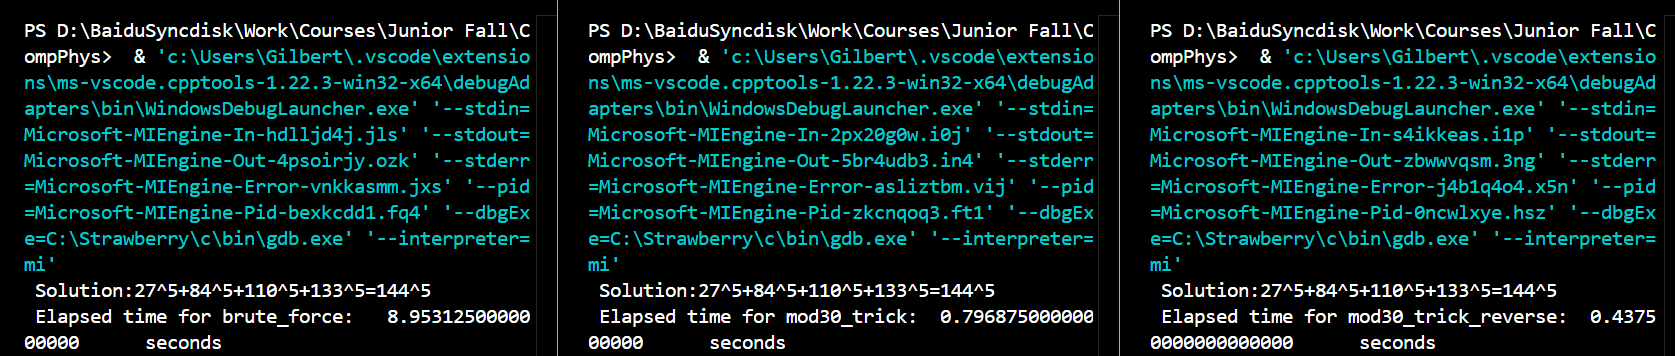
\includegraphics[width=1.0\textwidth]{Figs/comparison_f90.png}
    \caption{Fortran运行结果对比}
    \label{fig:output_f90}
\end{figure}

\begin{figure}[htp]
    \centering
    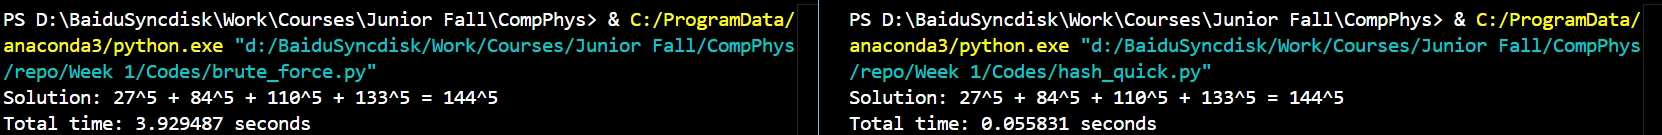
\includegraphics[width=1.0\textwidth]{Figs/comparison_py.png}
    \caption{Python运行结果对比}
    \label{fig:output_py}
\end{figure}
